Nos mercados eletrônicos modernos é possível a criação e envio de ordens digitais. No contexto do MM o principal tipo de ordem usado é a ordem limite. Uma ordem limite qualquer $o = (p, Q)$, onde $p$ é o valor da ordem e $Q$ é a quantidade ofertada. Para um intervalo de tempo discreto $t < T, t \in \mathbb{Z^{+}}$, onde $T$ é o momento do fechamento do mercado (ou final do pregão), o agente pode operar diversas vezes, atualizando os valores da ordem ao longo do tempo $t$. Para tal, identificar-se-há o preço e quantidade ofertada no tempo $t$ por $o_{t} \in \{o_{0}, ..., o_{T}\}$.

Como mencionado anteriormente, os \textit{LOB} são ordenados de acordo com as ofertas com melhores preços, sejam de compra ou venda. A diferença entre o preço da melhor oferta de compra e venda no livro para um determinado ativo é chamada de \textit{bid-ask spread}, representada por $\Delta = p^{(a, 0)} - p^{(b, 0)}$, onde $p^{(a, 0)}$ é o melhor $ask$ e $p^{(b, 0)}$ é o melhor \textit{bid}. Para um \textit{bid} (ou \textit{ask}) em uma posição qualquer, denota-se $p^{(b, i)}$, onde $i$ é a posição da oferta no \textit{LOB} ($p^{(i)}$ é decrescente para \textit{bids} e crescente para \textit{asks})

O objetivo de uma estratégia de \textit{market making} (\textit{MM}) nesse contexto é criar ofertas que superem as ordens existentes e venham a se tornar as melhores ofertas, tais que: 

\begin{itemize}
    \item $p^{(a, 0)} < p^{(a, MM)}$ para vendas;
    \item $p^{(b, 0)} > p^{(b, MM)}$ para compras;
\end{itemize}

onde $p^{(MM)}$ é o preço da oferta do agente e  $p^{(0)}$ é a melhor oferta existente.
É importante notar que quaisquer ordens criadas por um agente de \textit{MM} não geram novas transações no momento, ou seja, as ofertas de bid do agente não cruzam com ofertas de ask existentes e vice-versa. ($p^{(a, 0)} > p^{(b, MM)}$ e $p^{(b, 0)} < p^{(a, MM)}$ para novas ordens).

\begin{figure}[H]
	\begin{center}
		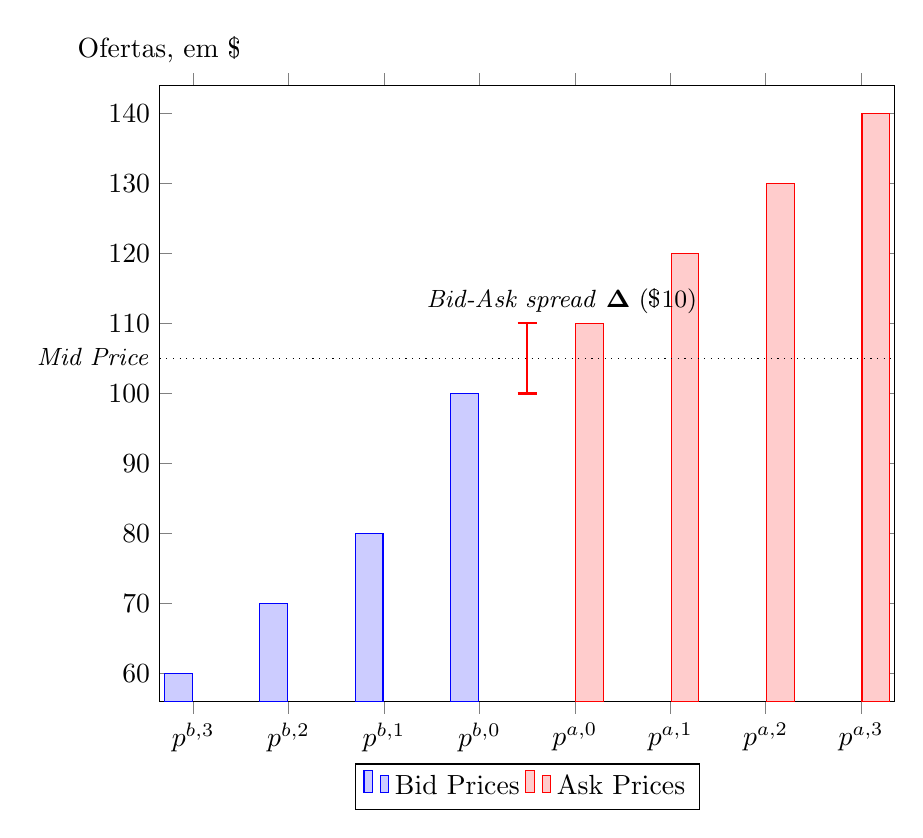
\begin{tikzpicture}
			\begin{axis}[
				x tick label style={/pgf/number format/1000 sep=},
				enlargelimits=0.05,
				legend style={at={(0.5,-0.1)}, anchor=north,legend columns=-1},
				ybar=0.7,
				ylabel={Ofertas, em \$},
    				ylabel style={
    				at={(0,1.02)},
    				anchor=south,
    				rotate=-90,
    			},
				width=0.9\textwidth, % Adjust the width to fit within the box
				xticklabels={
					$p^{b, 3}$, $p^{b, 2}$, $p^{b, 1}$, $p^{b, 0}$, 
					$p^{a, 0}$, $p^{a, 1}$, $p^{a, 2}$, $p^{a, 3}$
					},
				xtick={1,2,3,4,5,6,7,8}, % Set explicit tick positions
				after end axis/.code={
					\draw [red, thick, line cap=] (axis cs:4.5,100) -- (axis cs:4.5,110); % Static vertical line for spread with end caps
					\draw [red, thick] (axis cs:4.4,100) -- (axis cs:4.6,100);
					\draw [red, thick] (axis cs:4.4,110) -- (axis cs:4.6,110);
					\draw [black, dotted] (axis cs:0.65,105) -- (axis cs:8.35,105);
					\node[right, font=\small] at (rel axis cs:0.35,0.65) {\textit{Bid-Ask spread} $\mathbf{\Delta}$ (\$10)}; % Label for the spread line
					\node[left, font=\small] at (rel axis cs:0,0.56) {\textit{Mid Price}};
				}
				]
				% Represent bid prices in blue
				\addplot [blue, fill=blue!20] coordinates {(1, 60) (2, 70) (3, 80) (4, 100)};
				% Represent ask prices in red
				\addplot [red, fill=red!20] coordinates {(5, 110) (6, 120) (7, 130) (8, 140)};
				\legend{Bid Prices, Ask Prices}
			\end{axis}
		\end{tikzpicture}
	\end{center}
	\caption{Gráfico de ofertas de um livro de ordens limite $L$ qualquer}
\end{figure}

\begin{figure}[H]
	\begin{center}
		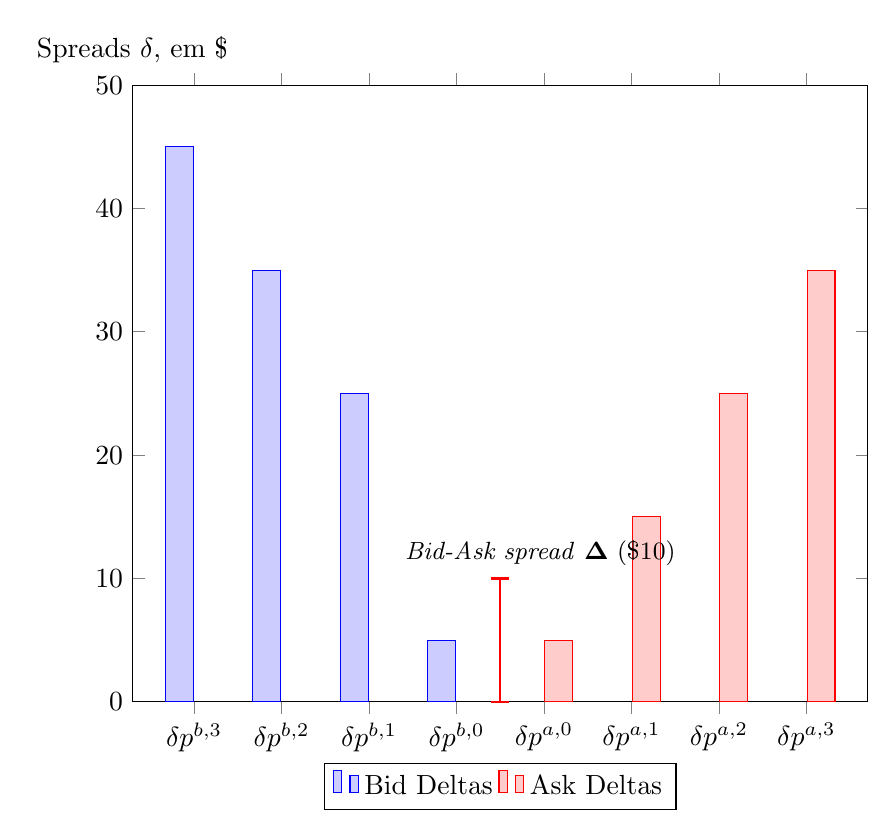
\begin{tikzpicture}
			\begin{axis}[
				x tick label style={/pgf/number format/1000 sep=},
				legend style={at={(0.5,-0.1)}, anchor=north,legend columns=-1},
				ybar=0.7,
				ylabel={Spreads $\delta$, em \$},
				ylabel style={
					at={(0,1.02)},
					anchor=south,
					rotate=-90,
				},
				ymin=0, ymax=50,
				width=0.9\textwidth, % Adjust the width to fit within the box
				xticklabels={
					$\delta p^{b, 3}$, $\delta p^{b, 2}$, $\delta p^{b, 1}$, $\delta p^{b, 0}$, 
					$\delta p^{a, 0}$, $\delta p^{a, 1}$, $\delta p^{a, 2}$, $\delta p^{a, 3}$
					},
				xtick={1,2,3,4,5,6,7,8}, % Set explicit tick positions
				after end axis/.code={
					\draw [red, thick, line cap=] (axis cs:4.5,0) -- (axis cs:4.5,10); 
					% Static vertical line for spread with end caps
					\draw [red, thick] (axis cs:4.4,0) -- (axis cs:4.6,0);
					\draw [red, thick] (axis cs:4.4,10) -- (axis cs:4.6,10);
					\node[right, font=\small] at (axis cs:3.3,12) {\textit{Bid-Ask spread} $\mathbf{\Delta}$ (\$10)}; % Label for the spread line
				}
				]
				% Represent bid prices in blue
				\addplot [blue, fill=blue!20] coordinates {(1, 45) (2, 35) (3, 25) (4, 5)};
				% Represent ask prices in red
				\addplot [red, fill=red!20] coordinates {(5, 5) (6, 15) (7, 25) (8, 35)};
				\legend{Bid Deltas, Ask Deltas}
			\end{axis}
		\end{tikzpicture}
	\end{center}
	\caption{Gráfico de spreads $\Delta$ de um livro de ordens limite $L$ qualquer}
\end{figure}

Para ilustrar melhor o funcionamento do livro de ordens considere a seguinte situação, para um único ativo: um agente qualquer de \textit{MM} tem a \textbf{única oferta de venda} pelo preço de $p^{(a, MM)}$ no mercado. Caso surja uma nova oferta de \textbf{compra} com melhor preço e acima do preço da oferta do agente $p^{(b, i)} \geq p^{(a, MM)}$, será gerada uma transação pelo preço $p^{(a, MM)}$ e a ordem de valor $p^{(b, i)}$ que gerou a transação é a ordem limite com preço de mercado. Após o motor de transações da bolsa receber a oferta $i$, uma transação ocorre e ambas ofertas são removidas do livro de ordens. 

O agente observa, para um determinado ativo e considerando novamente um índice de tempo discreto $t < T, t \in \mathbb{Z^{+}}$, três valores numéricos principais $(I_{t}, P_{t}, W_{t})$, sendo eles: 
\begin{itemize}
	\item o inventário $I_{t} \in \mathbb{Z}$ (a quantidade que têm do ativo);
	\item o preço médio do ativo $P_{t} \in \mathbb{R}$;
	\item o lucro financeiro do portfólio $W_{t} \in \mathbb{R}$;
	\item o valor total das negociações diárias, obtido a partir da expressão: $W_{t} + I_{t} \cdot P_{t}$;
\end{itemize}

A cada passo de tempo, ou seja, quando $t := t + 1$, o inventário do agente é atualizado da seguinte forma:
\begin{equation}
    \begin{aligned}
    	I_{t + 1} = N^{(b)}_{t + 1} - N^{(a)}_{t + 1} \label{eq:inventory}
    \end{aligned}
\end{equation}
onde $N^{(a)}$ e $N^{(b)}$ são as quantidades de ativos efetivamente vendidos ou comprados, distribuídas de acordo com um processo de contagem, com incrementos indepentes (note que os valores esperados dos incrementos dos processos seguem médias $\lambda_{t}^{(a)}$ e $\lambda_{t}^{(b)}$ que se alteram de acordo com o tempo $t$). Os incrementos dos processos de contagem são limitados externalmente à quantidade ofertada pelo agente, tal que $(N_{t + 1}^{(a)} - N_{t}^{(a)}) \leq Q_{t + 1}^{(a)}$ e $(N_{t + 1}^{(b)} - N_{t}^{(b)}) \leq Q_{t + 1}^{(b)}$.

O preço médio do ativo é facilmente obtido a partir de um movimento Browniano unidimensional (também chamado de processo de Wiener), de acordo com a equação incremental a seguir:
\begin{equation}
	\begin{aligned}
		P_{t+1} = P_t + \sigma \cdot \Delta Z_t
		\label{eq:midprice}
	\end{aligned}
\end{equation}
onde \(\sigma\) é a volatilidade do ativo e \(\Delta Z_t\) é uma variável aleatória amostrada de uma distribuição normal com média 0 e variância \(\Delta t\), onde \(\Delta t\) é o tamanho do intervalo de tempo discreto.

Por fim, o lucro financeiro do agente (também chamado de \textit{Profit and Loss} ou \textit{PnL}) é atualizado de acordo com a seguinte expressão:
\begin{equation}
	\begin{aligned}
		W_{t + 1} = W_{t} + p^{(a, MM)}_{t} \cdot (N^{(a)}_{t + 1} - N^{(a)}_{t}) - p^{(b, MM)}_{t} \cdot (N^{(b)}_{t + 1} - N^{(b)}_{t} )
		\label{eq:pnl}
	\end{aligned}
\end{equation}

A cada observação e atualização dos valores $(P_{t}, W_{t}, I_{t})$ o agente pode escolher não fazer nada ou realizar uma das ações abaixo:
\begin{enumerate}
    \item alterar as quantidades ofertadas $Q^{(a)}_{t + 1}$ e $Q^{(b)}_{t + 1}$;
    \item alterar os preços ofertados $p^{(a, MM)}_{t + 1}$ e $p^{(b, MM)}_{t + 1}$;
\end{enumerate}

O agente realiza essas mudanças buscando maximizar uma função-utilidade $U(X)$, que de preferência incorpore os valores do PnL, do inventário atual e do preço médio do ativo, assim como um fator de aversão ao risco. Para tal, definimos a progressão da recompensa $R$ em relação ao tempo $t$ como:

\begin{equation}
	\begin{aligned}
		R_{t + 1} = U(W_{t} + I_{t} \cdot P_{t})
		\label{eq:reward}
	\end{aligned}
\end{equation}

onde a função utilidade $U$ escolhida é exponencial, tal que $U(x) = -e^{-c x}$ e $c$ é o coeficiente de aversão ao risco.

Por fim, traduzindo os conceitos discutidos podem ser aplicado no contexto de aprendizado por reforço, formando o $MDP = (\mathcal{S}, \mathcal{A}, T_{a}, R_{a})$, onde o espaço de observações do ambiente é \(\mathcal{S} = \{(P, W, I) \mid P \in \mathbb{R}, W \in \mathbb{R}, I \in \mathbb{Z}\}\), o espaço de ações do agente é \(\mathcal{A} = \{(p^a, p^b, Q^a, Q^b) \mid p \in \mathbb{R}^+ \text{ e } Q \in \mathbb{N}\}\). Os valores do operador de transição $T$ são obtidos de acordo com as dinâmicas em \ref{eq:inventory}, \ref{eq:midprice} e \ref{eq:pnl} e os valores da função de recompensa é dada por \ref{eq:reward}.